\documentclass[12pt]{article}
\usepackage[utf8]{inputenc}
\usepackage{amsmath, amssymb}
\usepackage{xcolor}
\usepackage{geometry}
\usepackage{hyperref}
\usepackage{fancyhdr}
\usepackage{enumitem}
\usepackage{minted} % Code highlighting
\usepackage{booktabs} % Clean tables
\usepackage{tikz} % Optional for concept maps

\geometry{margin=1in}
\hypersetup{colorlinks=true, linkcolor=blue, urlcolor=cyan}

\pagestyle{fancy}
\fancyhf{}
\fancyhead[L]{\textbf{\TOPICTITLE}}
\fancyhead[R]{\thepage}

% -------------------------------
% Topic Metadata
% -------------------------------
\newcommand{\TOPICTITLE}{Application Layer: DNS and Network Applications}
\title{\TOPICTITLE\\\large Study-Ready Notes}
\author{Compiled by Andrew Photinakis}
\date{\today}

\setlength{\headheight}{15pt}

\begin{document}
\maketitle
\tableofcontents
\newpage

% This LaTeX file should be saved at: computer_networks/week02/application_layer_dns_network_applications.tex

\section{DNS: Domain Name System}
\subsection{Fundamental Concepts}

\begin{itemize}
    \item \textbf{People identifiers}: SSN, name, passport number
    \item \textbf{Internet host identifiers}:
          \begin{itemize}
              \item IP address (32-bit) - used for addressing datagrams
              \item Domain name (e.g., cs.umass.edu) - used by humans
          \end{itemize}
\end{itemize}

\textbf{Key Question}: How to map between IP addresses and domain names, and vice versa?

\subsection{DNS Definition and Characteristics}
\begin{itemize}
    \item \textbf{Distributed database} implemented in hierarchy of many name servers
    \item \textbf{Application-layer protocol}: hosts and DNS servers communicate to resolve names
    \item Core Internet function implemented as application-layer protocol
    \item Complexity resides at network's "edge"
\end{itemize}

\textcolor{blue}{[Summary: DNS is a distributed hierarchical system that translates human-readable domain names into machine-readable IP addresses, functioning as a critical Internet infrastructure component.]}

\section{DNS Services and Structure}
\subsection{DNS Services}

\begin{itemize}
    \item \textbf{Hostname-to-IP-address translation}: Primary function
    \item \textbf{Host aliasing}: Canonical vs. alias names
    \item \textbf{Mail server aliasing}: Email domain resolution
    \item \textbf{Load distribution}: Multiple IP addresses for one name (server replication)
\end{itemize}

\subsection{Why Not Centralize DNS?}
\begin{itemize}
    \item \textbf{Single point of failure}: Central server outage would break entire system
    \item \textbf{Traffic volume}: Immense query load would overwhelm single server
    \item \textbf{Distant centralized database}: High latency for remote users
    \item \textbf{Maintenance challenges}: Impossible to manage centrally at Internet scale
\end{itemize}

\textbf{Conclusion}: Centralization doesn't scale!

\textbf{Real-world scale evidence}:
\begin{itemize}
    \item Comcast DNS servers: 600 billion queries/day
    \item Akamai DNS servers: 2.2 trillion queries/day
\end{itemize}

\textcolor{orange}{[Mnemonic: DNS Problems - Single Traffic Distance Maintenance (STDM)]}
\textcolor{blue}{[Summary: DNS provides multiple services beyond basic name resolution, and its distributed nature solves scalability and reliability issues that would plague a centralized system.]}

\section{DNS Architecture and Characteristics}
\subsection{DNS System Properties}

\begin{itemize}
    \item \textbf{Humongous distributed database}: Approximately 1 billion records, each relatively simple
    \item \textbf{Massive query volume}: Handles many trillions of queries daily
          \begin{itemize}
              \item Many more reads than writes
              \item Performance critical: Milliseconds matter for user experience
              \item Almost every Internet transaction interacts with DNS
          \end{itemize}
    \item \textbf{Decentralized organization}: Millions of organizations responsible for their own records
    \item \textbf{"Bulletproof" requirements}: High reliability and security essential
\end{itemize}

\section{DNS Hierarchical Structure}
\subsection{Distributed Hierarchical Database}

% \begin{figure}[h]
%     \centering
%     \begin{tikzpicture}[scale=0.8]
%         \node[draw, rectangle] (root) at (0,4) {Root DNS Servers};
%         \node[draw, rectangle] (tld1) at (-4,2) {.com DNS servers};
%         \node[draw, rectangle] (tld2) at (-2,2) {.org DNS servers};
%         \node[draw, rectangle] (tld3) at (0,2) {.edu DNS servers};
%         \node[draw, rectangle] (tld4) at (2,2) {...};
%         \node[draw, rectangle] (auth1) at (-4,0) {yahoo.com DNS servers};
%         \node[draw, rectangle] (auth2) at (-2,0) {amazon.com DNS servers};
%         \node[draw, rectangle] (auth3) at (0,0) {umass.edu DNS servers};
%         \node[draw, rectangle] (auth4) at (2,0) {nyu.edu DNS servers};
%         \node[draw, rectangle] (auth5) at (4,0) {pbs.org DNS servers};

%         \draw[->] (root) -- (tld1);
%         \draw[->] (root) -- (tld2);
%         \draw[->] (root) -- (tld3);
%         \draw[->] (root) -- (tld4);
%         \draw[->] (tld1) -- (auth1);
%         \draw[->] (tld1) -- (auth2);
%         \draw[->] (tld3) -- (auth3);
%         \draw[->] (tld3) -- (auth4);
%         \draw[->] (tld2) -- (auth5);
%     \end{tikzpicture}
%     \caption{DNS Hierarchical Database Structure}
%     \label{fig:dns_hierarchy}
% \end{figure}

\begin{figure}[htbp]
    \centering
    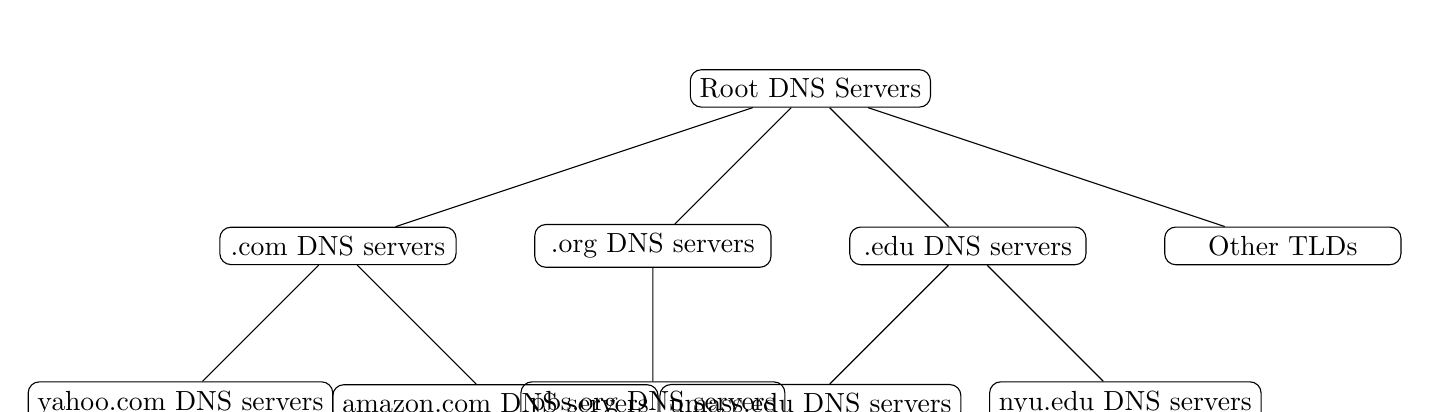
\begin{tikzpicture}[
            level distance=2cm,
            sibling distance=4cm,
            every node/.style={draw, rectangle, rounded corners, align=center, minimum width=3cm}
        ]
        % Root node
        \node {Root DNS Servers}
        % Level 1: TLDs
        child { node {.com DNS servers}
                % Level 2: Authoritative
                child { node {yahoo.com DNS servers} }
                child { node {amazon.com DNS servers} }
            }
        child { node {.org DNS servers}
                child { node {pbs.org DNS servers} }
            }
        child { node {.edu DNS servers}
                child { node {umass.edu DNS servers} }
                child { node {nyu.edu DNS servers} }
            }
        child { node {Other TLDs} };
    \end{tikzpicture}
    \caption{DNS Hierarchical Database Structure}
    \label{fig:dns_hierarchy}
\end{figure}


\textbf{Resolution process example}: Client wants IP address for www.amazon.com
\begin{enumerate}
    \item Client queries root server to find .com DNS server
    \item Client queries .com DNS server to get amazon.com DNS server
    \item Client queries amazon.com DNS server to get IP address for www.amazon.com
\end{enumerate}

\textcolor{blue}{[Summary: DNS uses a hierarchical distributed database with root servers at the top, TLD servers in the middle, and authoritative servers at the bottom for specific domains.]}

\section{DNS Server Types}
\subsection{Root Name Servers}

\begin{itemize}
    \item Official contact-of-last-resort for unresolved names
    \item Incredibly important Internet function - Internet couldn't function without it!
    \item DNSSEC provides security (authentication, message integrity)
    \item Managed by ICANN (Internet Corporation for Assigned Names and Numbers)
\end{itemize}

\textbf{Deployment statistics}:
\begin{itemize}
    \item 13 logical root name "servers" worldwide
    \item Each "server" replicated many times (~200 servers in US)
    \item Geographic distribution for reliability and performance
\end{itemize}

\subsection{Top-Level Domain (TLD) Servers}
\begin{itemize}
    \item Responsible for top-level domains:
          \begin{itemize}
              \item Generic TLDs: .com, .org, .net, .edu, .aero, .jobs, .museums
              \item Country-code TLDs: .cn, .uk, .fr, .ca, .jp
          \end{itemize}
    \item Managed by specific organizations:
          \begin{itemize}
              \item Network Solutions: authoritative registry for .com, .net
              \item Educause: .edu TLD
          \end{itemize}
\end{itemize}

\subsection{Authoritative DNS Servers}
\begin{itemize}
    \item Organization's own DNS server(s)
    \item Provide authoritative hostname-to-IP mappings for organization's named hosts
    \item Can be maintained by organization or service provider
\end{itemize}

\subsection{Local DNS Name Servers}
\begin{itemize}
    \item First point of contact for host DNS queries
    \item Returns replies from:
          \begin{itemize}
              \item Local cache of recent name-to-address translations
              \item Forwarding requests into DNS hierarchy for resolution
          \end{itemize}
    \item Each ISP has local DNS name server
    \item Doesn't strictly belong to hierarchy
\end{itemize}

\textbf{Finding your local DNS server}:
\begin{itemize}
    \item MacOS: \texttt{\% scutil --dns}
    \item Windows: \texttt{> ipconfig /all}
\end{itemize}

\textcolor{teal}{[Concept Map: DNS Hierarchy → Root → TLD → Authoritative → Local (caching)]}
\textcolor{blue}{[Summary: DNS uses four main server types: root servers for global coordination, TLD servers for domain categories, authoritative servers for specific domains, and local servers for client-side caching and resolution.]}

\section{DNS Name Resolution Methods}
\subsection{Iterated Query}

\begin{figure}[htbp]
    \centering
    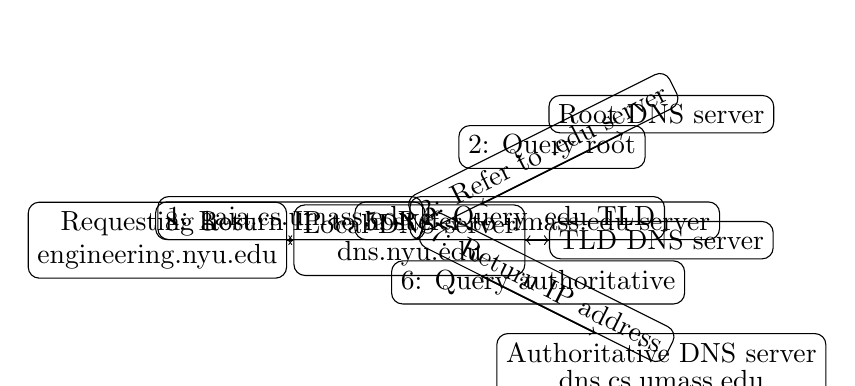
\begin{tikzpicture}[scale=0.8, every node/.style={draw, rectangle, rounded corners, align=center}]
        % Nodes
        \node (host) at (0,0) {\shortstack{Requesting host\\engineering.nyu.edu}};
        \node (local) at (4,0) {\shortstack{Local DNS server\\dns.nyu.edu}};
        \node (root) at (8,2) {Root DNS server};
        \node (tld) at (8,0) {TLD DNS server};
        \node (auth) at (8,-2) {\shortstack{Authoritative DNS server\\dns.cs.umass.edu}};

        % Arrows
        \draw[->] (host) -- node[above] {1: gaia.cs.umass.edu} (local);
        \draw[->] (local) -- node[above] {2: Query root} (root);
        \draw[->] (root) -- node[sloped, above] {3: Refer to .edu server} (local);
        \draw[->] (local) -- node[above] {4: Query .edu TLD} (tld);
        \draw[->] (tld) -- node[sloped, above] {5: Refer to umass.edu server} (local);
        \draw[->] (local) -- node[above] {6: Query authoritative} (auth);
        \draw[->] (auth) -- node[sloped, above] {7: Return IP address} (local);
        \draw[->] (local) -- node[above] {8: Return IP to host} (host);
    \end{tikzpicture}
    \caption{DNS Iterated Query Resolution}
    \label{fig:iterated_query}
\end{figure}



\textbf{Characteristics}:
\begin{itemize}
    \item Contacted server replies with name of server to contact
    \item "I don't know this name, but ask this server"
    \item Local server does most of the work
\end{itemize}

\subsection{Recursive Query}

\begin{figure}[h]
    \centering
    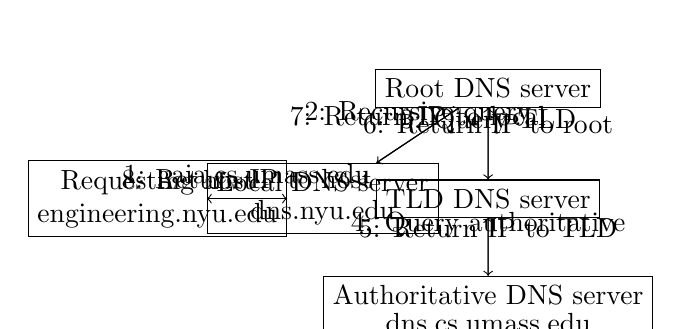
\begin{tikzpicture}[scale=0.7]
        \node[draw] (host) at (0,0) {\shortstack{Requesting host\\engineering.nyu.edu}};
        \node[draw] (local) at (3,0) {\shortstack{Local DNS server\\dns.nyu.edu}};
        \node[draw] (root) at (6,2) {Root DNS server};
        \node[draw] (tld) at (6,0) {TLD DNS server};
        \node[draw] (auth) at (6,-2) {\shortstack{Authoritative DNS server\\dns.cs.umass.edu}};

        \draw[->] (host) -- node[above] {1: gaia.cs.umass.edu} (local);
        \draw[->] (local) -- node[above] {2: Recursive query} (root);
        \draw[->] (root) -- node[above] {3: Query TLD} (tld);
        \draw[->] (tld) -- node[above] {4: Query authoritative} (auth);
        \draw[->] (auth) -- node[above] {5: Return IP to TLD} (tld);
        \draw[->] (tld) -- node[above] {6: Return IP to root} (root);
        \draw[->] (root) -- node[above] {7: Return IP to local} (local);
        \draw[->] (local) -- node[above] {8: Return IP to host} (host);
    \end{tikzpicture}
    \caption{DNS Recursive Query Resolution}
    \label{fig:recursive_query}
\end{figure}

\textbf{Characteristics}:
\begin{itemize}
    \item Puts burden of name resolution on contacted name server
    \item Potential heavy load at upper levels of hierarchy
    \item Less common in practice due to load concerns
\end{itemize}

\textcolor{blue}{[Summary: DNS supports two resolution methods - iterated queries where servers refer clients to other servers, and recursive queries where servers do the complete resolution on behalf of clients.]}

\section{DNS Caching and Performance}
\subsection{Caching DNS Information}

\begin{itemize}
    \item Once any name server learns mapping, it \textbf{caches} the mapping
    \item Immediately returns cached mapping for subsequent queries
    \item \textbf{Benefits}:
          \begin{itemize}
              \item Improves response time significantly
              \item Reduces load on DNS infrastructure
          \end{itemize}
    \item \textbf{Time-to-Live (TTL)}:
          \begin{itemize}
              \item Cache entries timeout after TTL expires
              \item TLD servers typically cached in local name servers
          \end{itemize}
\end{itemize}

\subsection{Cache Limitations}
\begin{itemize}
    \item Cached entries may be \textbf{out-of-date}
    \item If host changes IP address, may not be known Internet-wide until all TTLs expire
    \item DNS provides \textbf{best-effort name-to-address translation}
\end{itemize}

\textcolor{orange}{[Mnemonic: DNS Cache - Time To Live, Temporarily Local, Limited freshness]}
\textcolor{blue}{[Summary: DNS caching dramatically improves performance but introduces potential staleness issues, with TTL values controlling how long cached entries remain valid.]}

\section{DNS Records and Protocol}
\subsection{DNS Resource Records (RR)}

DNS: distributed database storing resource records (RR)

\textbf{RR format}: \{name, value, type, ttl\}

\begin{itemize}
    \item \textbf{type=A}
          \begin{itemize}
              \item Name: hostname
              \item Value: IP address
          \end{itemize}

    \item \textbf{type=CNAME}
          \begin{itemize}
              \item Name: alias name for canonical name
              \item Value: canonical name
              \item Example: www.ibm.com is really servereast.backup2.ibm.com
          \end{itemize}

    \item \textbf{type=NS}
          \begin{itemize}
              \item Name: domain (e.g., foo.com)
              \item Value: hostname of authoritative name server for this domain
          \end{itemize}

    \item \textbf{type=MX}
          \begin{itemize}
              \item Value: name of SMTP mail server associated with name
          \end{itemize}
\end{itemize}

\subsection{DNS Protocol Messages}

DNS query and reply messages share the same format:

\begin{table}[h]
    \centering
    \begin{tabular}{|l|l|}
        \hline
        \textbf{Field}    & \textbf{Description}                                    \\
        \hline
        Identification    & 16-bit number for query/reply matching                  \\
        \hline
        Flags             & Query/reply, recursion desired/available, authoritative \\
        \hline
        \# Questions      & Number of questions in question section                 \\
        \hline
        \# Answer RRs     & Number of answer resource records                       \\
        \hline
        \# Authority RRs  & Number of authority resource records                    \\
        \hline
        \# Additional RRs & Number of additional resource records                   \\
        \hline
        Questions         & Variable number of questions (name, type fields)        \\
        \hline
        Answers           & Variable number of RRs in response to query             \\
        \hline
        Authority         & Records for authoritative servers                       \\
        \hline
        Additional Info   & Additional "helpful" information                        \\
        \hline
    \end{tabular}
    \caption{DNS Message Format}
    \label{tab:dns_message}
\end{table}

\textcolor{blue}{[Summary: DNS uses standardized resource records to store different types of information and employs a consistent message format for both queries and replies with multiple sections for different purposes.]}

\section{DNS Administration and Security}
\subsection{Registering Domain Information}

\textbf{Example}: New startup "Network Utopia"

\begin{enumerate}
    \item Register name networkingtopia.com at DNS registrar (e.g., Network Solutions)
    \item Provide names and IP addresses of authoritative name servers (primary and secondary)
    \item Registrar inserts NS and A records into .com TLD server:
          \begin{itemize}
              \item (networkingpia.com, dns1.networkingpia.com, NS)
              \item (dns1.networkingpia.com, 212.212.212.1, A)
          \end{itemize}
    \item Create authoritative server locally with IP address 212.212.212.1
          \begin{itemize}
              \item Type A record for www.networkingtopia.com
              \item Type MX record for networkingpia.com
          \end{itemize}
\end{enumerate}

\subsection{DNS Security Threats}
\subsubsection{DDoS Attacks}
\begin{itemize}
    \item Bombard root servers with traffic
    \item Not successful to date due to:
          \begin{itemize}
              \item Traffic filtering
              \item Local DNS servers cache TLD server IPs, allowing root server bypass
          \end{itemize}
    \item Bombarding TLD servers potentially more dangerous
\end{itemize}

\subsubsection{Spoofing Attacks}
\begin{itemize}
    \item Intercept DNS queries, returning bogus replies
    \item DNS cache poisoning
    \item Countermeasure: DNSSEC (RFC 4033) provides authentication services
\end{itemize}

\textcolor{blue}{[Summary: DNS administration involves registering domains with registrars who update TLD servers, while DNS security addresses DDoS and spoofing attacks through filtering, caching, and DNSSEC authentication.]}

\section*{Exam Questions}

\subsection*{DNS Fundamentals}
\begin{enumerate}
    \item Explain why DNS uses a distributed hierarchical architecture instead of a centralized system. List at least three reasons.
    \item Compare and contrast iterative and recursive DNS query resolution methods. What are the advantages and disadvantages of each?
    \item Describe the four main types of DNS servers in the hierarchy and their respective roles.
\end{enumerate}

\subsection*{DNS Operations}
\begin{enumerate}
    \item Walk through the complete process of resolving www.example.com using iterative queries, naming each server type involved.
    \item Explain how DNS caching improves performance and what problem it introduces regarding record freshness.
    \item What is TTL in DNS and why is it important for both performance and reliability?
\end{enumerate}

\subsection*{DNS Records and Security}
\begin{enumerate}
    \item Compare DNS A records, CNAME records, NS records, and MX records. Provide an example use case for each.
    \item Describe two major types of DNS security attacks and the countermeasures used against them.
    \item Explain the process of registering a new domain name and getting it into the DNS system.
\end{enumerate}

\textcolor{red}{[Exam Questions: These questions cover DNS architecture, operations, record types, and security - key areas for understanding how the Domain Name System works in practice.]}

\end{document}